\حصہ{\عددی{x\to \mp \infty} پر حد، متقارب اور   غالب اجزاء}
اس حصہ میں  ناطق تفاعل (دو کثیر رکنیوں کے حاصل تقسیم)  کے علاوہ دیگر تفاعل، جن کا \عددی{x\to \mp \infty} پر دلچسپ حد ہو، کی ترسیمات پر  متقارب اور غالب اجزاء کی مدد سے   غور کیا جائے گا۔

\جزوحصہء{\عددی{x\to \mp \infty} پر حد}
تفاعل \عددی{f(x)=\tfrac{1}{x}} تمام \عددی{x\ne 0} کے لئے معین ہے۔ مثبت اور بتدریج بڑھتی \عددی{x}  کے لئے \عددی{\tfrac{1}{x}} کی قیمت بتدریج  گھٹے گی۔ منفی \عددی{x} جس کی مقدار بتدریج بڑھتی ہو  کے لئے \عددی{\tfrac{1}{x}} کی مقدار بتدریج  گھٹے گی۔ ہم مختصراً کہتے ہیں کہ \عددی{x\to\mp\infty} پر \عددی{f(x)=\tfrac{1}{x}} کا حد \عددی{0} ہے۔ 
\begin{figure}
\centering
\begin{tikzpicture}
\begin{axis}[small,axis lines=middle,xlabel={$x$},ylabel={$y$},xmax=4.9,xlabel style={at={(current axis.right of origin)},anchor=west},ylabel style={at={(current axis.above origin)},anchor=south}]
\addplot[domain=-4:-0.22]{1/x};
\addplot[domain=0.22:4]{1/x}node[above left]{$y=\tfrac{1}{x}$};
\end{axis}
\end{tikzpicture}
\caption{تفاعل \عددی{y=\tfrac{1}{x}} کی ترسیم۔}
\label{شکل_استعمال_حد_معکوس_ترسیم}
\end{figure}

\ابتدا{تعریف}
\begin{enumerate}[1.]
\item
اگر ہر عدد \عددی{\epsilon>0} کے لئے ایسا مطابقتی عدد \عددی{M} موجود ہو کہ تمام \عددی{x>M}  کے لئے \عددی{\abs{f(x)-L}<\epsilon} ہو یعنی
\begin{align*}
x>M\quad \implies \quad \abs{f(x)-L}<\epsilon
\end{align*}
 تب ہم کہتے ہیں کہ \عددی{x} لامتناہی تک پہنچنے پر  \عددی{f(x)} کا حد \عددی{L} ہے جس کو ہم
\begin{align*}
\lim_{x\to\infty} f(x)=L
\end{align*}
لکھتے ہیں۔
\item
اگر ہر عدد \عددی{\epsilon>0} کے لئے ایسا مطابقتی عدد \عددی{N} موجود ہو کہ تمام \عددی{x<N}  کے لئے \عددی{\abs{f(x)-L}<\epsilon} ہو یعنی
\begin{align*}
x<N\quad \implies \quad \abs{f(x)-L}<\epsilon
\end{align*}
 تب ہم کہتے ہیں کہ \عددی{x} منفی لامتناہی تک پہنچنے پر  \عددی{f(x)} کا حد \عددی{L} ہے جس کو ہم
\begin{align*}
\lim_{x\to-\infty} f(x)=L
\end{align*}
لکھتے ہیں۔

\end{enumerate}
\انتہا{تعریف}
%===========================

لامتناہی کو \عددی{\infty} سے ظاہر کیا جاتا ہے جو حقیقی عدد نہیں ہے لہٰذا اس کو حساب میں عام اعداد کی طرح استعمال نہیں کیا جا سکتا ہے۔ 

\عددی{x\to \mp \infty} پر تفاعل کا حد تلاش کرنے کی حکمت عملی وہی ہے جو حصہ \حوالہ{حصہ_حد_قواعد} میں استعمال کی گئی۔ وہاں ہم نے مستقل تفاعل \عددی{y=k} اور مماثل تفاعل \عددی{y=x} کے حد حاصل کیے۔اس کے بعد الجبرائی ملاپ کا ایک مسئلہ استعمال کرتے ہوئے ان نتائج سے دیگر تفاعل کے حد حاصل کیے گئے۔ یہاں ابتدائی تفاعل کو \عددی{y=k} اور \عددی{y=x} کی بجائے \عددی{y=k} اور \عددی{y=\tfrac{1}{x}} لیتے ہوئے ہم یہی کچھ دوبارہ کرتے ہیں۔ 

با ضابطہ  تعریف استعمال کرتے ہوئے ہمیں درج ذیل ثابت کرنا ہو گا۔
\begin{align}\label{مساوات_استعمال_معکوس_حد}
\lim_{x\to \mp \infty} k=k,\quad \lim_{x\to \mp \infty}\frac{1}{x}=0
\end{align}
ہم مستقل تفاعل کا حد سوال کے لئے  رکھتے ہیں جبکہ دوسرے تفاعل کو یہاں ثابت کرتے ہیں۔

\ابتدا{مثال}\شناخت{مثال_استعمال_حد_معکوس_ترسیم_ثبوت}
درج ذیل دکھائیں۔
\begin{multicols}{2}
\begin{enumerate}[a.]
\item
$\lim_{x\to\infty}\frac{1}{x}=0$
\item
$\lim_{x\to -\infty}\frac{1}{x}=0$
\end{enumerate}
\end{multicols}
حل:
\begin{enumerate}[a.]
\item
فرض کریں \عددی{\epsilon>0} دیا گیا ہے۔ہمیں ایسا عدد \عددی{M} تلاش کرنے ہے کہ تمام \عددی{x} کے لئے درج ذیل مطمئن ہوتا ہو۔
\begin{align*}
x>M,\quad \implies \quad \abs{\frac{1}{x}-0}=\abs{\frac{1}{x}}<\epsilon
\end{align*}
\عددی{M=\tfrac{1}{\epsilon}} یا اس سے بڑا مثبت عدد منتخب کرنے سے درج بالا مطمئن ہوتا ہے۔ یوں \عددی{\lim_{x\to\infty}\tfrac{1}{x}=0} ثابت ہوتا ہے (شکل \حوالہ{شکل_مثال_استعمال_حد_معکوس_ترسیم_ثبوت})۔
\item
فرض کریں \عددی{\epsilon>0} دیا گیا ہے۔ہمیں ایسا عدد \عددی{N} تلاش کرنے ہے کہ تمام \عددی{x} کے لئے درج ذیل مطمئن ہوتا ہو۔
\begin{align*}
x<N,\quad \implies \quad \abs{\frac{1}{x}-0}=\abs{\frac{1}{x}}<\epsilon
\end{align*}
\عددی{N=-\tfrac{1}{\epsilon}} یا \عددی{-\tfrac{1}{\epsilon}} سے کم منتخب کرنے سے درج بالا مطمئن ہوتا ہے۔ یوں \عددی{\lim_{x\to-\infty}\tfrac{1}{x}=0} ثابت ہوتا ہے (شکل \حوالہ{شکل_مثال_استعمال_حد_معکوس_ترسیم_ثبوت})۔
\end{enumerate}
%
\begin{figure}
\centering
\begin{tikzpicture}[font=\small]
\begin{axis}[clip=false,small,axis lines=middle,xlabel={$x$},ylabel={$y$},xlabel style={at={(current axis.right of origin)},anchor=west},ylabel style={at={(current axis.above origin)},anchor=south},xtick={-1,1},xticklabels={,},ytick={-1,1},yticklabels={,$\epsilon$}]
\addplot[domain=-2:-0.5]{1/x};
\addplot[domain=0.5:2]{1/x};
\draw(axis cs:-1,1)node[]{$y=\tfrac{1}{x}$};
\draw[dashed](0,1)--(2,1)node[right]{$y=\epsilon$}  (1,1)--(1,0)node[below]{$M=\tfrac{1}{\epsilon}$};
\draw[dashed](0,-1)node[right,font=\scriptsize]{$-\epsilon$}--(-2,-1)   (-1,-1)--(-1,0)node[above]{$N=-\tfrac{1}{\epsilon}$};
\draw[stealth-] (axis cs:1.75,0)--(axis cs:1.75,-0.5);
\draw[stealth-](axis cs:1.75,1)--(axis cs:1.75,1.5)node[above,align=right]{\RL{کسی بھی \عددی{\epsilon} کے لئے }\\   \RL{\عددی{x=\tfrac{1}{\epsilon}} پر ترسیم اس}\\   \RL{خطہ میں داخل ہوتی ہے}};
\draw[stealth-] (axis cs:-1.75,0)--(axis cs:-1.75,-0.5);
\draw[stealth-](axis cs:-1.75,-1)--(axis cs:-1.75,-1.5)node[below,align=right]{\RL{کسی بھی \عددی{\epsilon} کے لئے }\\   \RL{\عددی{x=-\tfrac{1}{\epsilon}} پر ترسیم اس}\\   \RL{خطہ میں داخل ہوتی ہے}};
\end{axis}
\end{tikzpicture}
\caption{حد کی تلاش میں جیومیٹری (مثال \حوالہ{مثال_استعمال_حد_معکوس_ترسیم_ثبوت})}
\label{شکل_مثال_استعمال_حد_معکوس_ترسیم_ثبوت}
\end{figure}

\انتہا{مثال}
%=========================

مساوات \حوالہ{مساوات_استعمال_معکوس_حد} کو استعمال کرتے ہوئے درج ذیل مسئلہ سے ہم دیگر حل تلاش کر سکتے ہیں۔

\ابتدا{مسئلہ}\موٹا{\عددی{x\to\mp\infty} پر حل کے خواص}\\
اگر \عددی{\lim_{x\to\mp\infty}f(x)=L} اور \عددی{\lim_{x\to\mp\infty}g(x)=M} ہوں تب درج ذیل درست ہوں گے۔ (\عددی{L} اور \عددی{M} حقیقی اعداد ہیں۔)
\begin{description}
\item[قاعدہ مجموعہ:]\quad
$\lim_{x\to \mp\infty}[f(x)+g(x)]=L+M$
\item[قاعدہ فرق:]\quad
$\lim_{x\to \mp\infty}[f(x)-g(x)]=L-M$
\item[قاعدہ ضرب:]\quad
$\lim_{x\to \mp\infty}f(x)\cdot g(x)=L\cdot M$
\item[قاعدہ ضرب مستقل:]\quad
$\lim_{x\to \mp\infty}k f(x)=kL$
\item[قاعدہ حاصل تقسیم:]\quad
$\lim_{x\to \mp\infty} \frac{f(x)}{g(x)}=\frac{L}{M}$
\item[قاعدہ طاقت:]\quad
اگر \عددی{m} اور \عددی{n} عدد صحیح ہوں تب
$\lim_{x\to \mp\infty}[f(x)]^{m/n}=L^{m/n}$
\end{description}
\انتہا{مسئلہ}
%========================

یہ خواص بالکل مسئلہ \حوالہ{مسئلہ_حد_قواعد-الف} (صفحہ \حوالہصفحہ{مسئلہ_حد_قواعد-الف}) میں دیے گئے خواص کی طرح ہیں اور انہیں ہم بالکل اسی طرح استعمال کرتے ہیں۔

\ابتدا{مثال}
\begin{enumerate}[a.]
\item
\begin{align*}
\lim_{x\to \infty}(5+\tfrac{1}{x})&=\lim_{x\to\infty} 5+\lim_{x\to\infty}\tfrac{1}{x}&&\text{\RL{قاعدہ مجموعہ}}\\
&=5+0=5&&\text{\RL{معلوم قیمتیں}}
\end{align*}
\item
\begin{align*}
\lim_{x\to-\infty}\frac{\pi\sqrt{3}}{x^2}&=\lim_{x\to-\infty}\pi\sqrt{3}\cdot \frac{1}{x}\cdot \frac{1}{x}\\
&=\lim_{x\to-\infty}\pi\sqrt{3}\cdot\lim_{x\to-\infty}\frac{1}{x}\cdot\lim_{x\to-\infty}\frac{1}{x}&&\text{\RL{قاعدہ ضرب}}\\
&=\pi\sqrt{3}\cdot 0 \cdot 0=0&&\text{\RL{معلوم قیمتیں}}
\end{align*}
\end{enumerate}
\انتہا{مثال}
%========================
\ابتدا{مثال}\شناخت{مثال_استعمال_حد_لا_متناہی_الف}\ترچھا{شمار کنندہ اور نسب نما میں بلند تر طاقت ایک جیسے ہیں} (شکل \حوالہ{شکل_مثال_استعمال_حد_لا_متناہی_الف})
\begin{align*}
\lim_{x\to\infty} \frac{5x^2+8x-3}{3x^2+2}&=\lim_{x\to\infty}\frac{5+\tfrac{8}{x}-\tfrac{3}{x^2}}{3+\tfrac{2}{x^2}}&&\text{\RL{شمار کنندہ اور نسب نما کو \عددی{x^2} سے تقسیم کریں}}\\
&=\frac{5+0-0}{3+0}=\frac{5}{3}
\end{align*}
%
\begin{figure}
\centering
\begin{minipage}{0.45\textwidth}
\centering
\begin{tikzpicture}
\begin{axis}[clip=false,small,axis lines=middle,xlabel={$x$},ylabel={$y$},xlabel style={at={(current axis.right of origin)},anchor=west},ylabel style={at={(current axis.above origin)},anchor=south}]
\addplot[domain=-5:10.5,smooth]{(5*x^2+8*x-3)/(3*x^2+2)}node[above left,yshift=2mm]{$y=\tfrac{5x^2+8x-3}{3x^2+2}$};
\addplot[domain=-5:10]{5/3}node[pos=0.6,pin=-45:{$y=\tfrac{5}{3}$}]{};
\end{axis}
\end{tikzpicture}
\caption{ترسیم تفاعل اور حد (مثال \حوالہ{مثال_استعمال_حد_لا_متناہی_الف})}
\label{شکل_مثال_استعمال_حد_لا_متناہی_الف}
\end{minipage}\hfill
\begin{minipage}{0.45\textwidth}
\centering
\begin{tikzpicture}
\begin{axis}[clip=false,small,axis lines=middle,xlabel={$x$},ylabel={$y$},xlabel style={at={(current axis.right of origin)},anchor=west},ylabel style={at={(current axis.above origin)},anchor=south}]
\addplot[domain=-4.25:0.5,smooth]{(11*x+2)/(2*x^3-1)};
\addplot[domain=1:5.9,smooth]{(11*x+2)/(2*x^3-1)}node[above left,yshift=2mm]{$y=\tfrac{11x+2}{2x^3-1}$};
\draw(axis cs:0.793,-10)--(axis cs:0.793,12);
\end{axis}
\end{tikzpicture}
\caption{ترسیم تفاعل اور حد (مثال \حوالہ{مثال_استعمال_حد_لا_متناہی_ب})}
\label{شکل_مثال_استعمال_حد_لا_متناہی_ب}
\end{minipage}\hfill
\end{figure}
\انتہا{مثال}
%=====================
\ابتدا{مثال}\شناخت{مثال_استعمال_حد_لا_متناہی_ب}\ترچھا{شمار کنندہ کی بلند ترین طاقت نسب نما کی بلند ترین طاقت سے کم ہے} (شکل \حوالہ{شکل_مثال_استعمال_حد_لا_متناہی_ب})
\begin{align*}
\lim_{x\to -\infty}\frac{11x+2}{2x^3-1}&=\lim_{x\to-\infty}\frac{\tfrac{11}{x^2}+\tfrac{2}{x^3}}{2-\tfrac{1}{x^3}}&&\text{\RL{شمار کنندہ اور نسب نما کو \عددی{x^3} سے تقسیم کریں}}\\
&=\frac{0+0}{2-0}=0
\end{align*}
\انتہا{مثال}

%===========================
\ابتدا{مثال}\شناخت{مثال_استعمال_حد_لا_متناہی_ج}\ترچھا{شمار کنندہ کی بلند ترین طاقت نسب نما کی بلند ترین طاقت سے زیادہ ہے۔} شکل \حوالہ{شکل_مثال_استعمال_حد_لا_متناہی_ج} 
\begin{enumerate}[a.]
\item
\begin{align*}
\lim_{x\to -\infty}\frac{2x^2-3}{7x+4}&=\lim_{x\to-\infty}\frac{2x-\tfrac{3}{x}}{7+\tfrac{4}{x}}&&\text{\RL{شمار کنندہ اور نسب نما کو \عددی{x} سے تقسیم کریں}}\\
&=-\infty
\end{align*}
\item
\begin{align*}
\lim_{x\to-\infty}\frac{-4x^3+7x}{2x^2-3x-10}&=\lim_{x\to-\infty}\frac{-4x+\tfrac{7}{x}}{2-\tfrac{3}{x}-\tfrac{10}{x^2}}&&\text{\RL{شمار کنندہ اور نسب نما کو \عددی{x^2} سے تقسیم کریں}}\\
&=\frac{\infty}{2}=\infty
\end{align*}
\end{enumerate}
\انتہا{مثال}
%===========================
\begin{figure}
\centering
\begin{minipage}{0.45\textwidth}
\centering
\begin{tikzpicture}
\pgfmathsetmacro{\k}{-4/7}
\begin{axis}[small,axis lines=middle,xlabel={$x$},ylabel={$y$}]
\addplot[domain=-5:\k-0.2,smooth]{(2*x^2-3)/(7*x+4)};
\addplot[domain=\k-0.2:\k-0.1,smooth]{(2*x^2-3)/(7*x+4)};
\addplot[domain=\k+0.1:\k+0.2,smooth]{(2*x^2-3)/(7*x+4)};
\addplot[domain=\k+0.2:4.2,smooth]{(2*x^2-3)/(7*x+4)}node[above left]{$y=\tfrac{2x^2-3}{7x+4}$};
\addplot[] plot coordinates {(\k,-4) (\k,3)};
\end{axis}
\end{tikzpicture}
\caption{ترسیم برائے مثال \حوالہ{مثال_استعمال_حد_لا_متناہی_ج}}
\label{شکل_مثال_استعمال_حد_لا_متناہی_ج}
\end{minipage}\hfill
\begin{minipage}{0.45\textwidth}
\centering
\begin{tikzpicture}[font=\small]
\begin{axis}[small,axis lines=middle,xlabel={$x$},ylabel={$y$},xtick={\empty},ytick={\empty},xlabel style={at={(current axis.right of origin)},anchor=west},ylabel style={at={(current axis.above origin)},anchor=south},axis line style=thick]
\addplot[domain=-4:-0.25]{1/x};
\addplot[domain=0.25:4]{1/x}node[pos=0.5,above right]{$y=\tfrac{1}{x}$};
\draw(axis cs:2.5,0)node[below,align=center]{\RL{افقی متقارب}\\ $y=0$ };
\draw(axis cs:-2,0)node[above]{\RL{افقی متقارب}};
\draw(axis cs:0,-2)node[below,rotate=90]{\RL{انتصابی متقارب}};
\draw(axis cs:0,2.5)node[above,rotate=90,align=center]{\RL{انتصابی متقارب}\\ $x=0$  };
\end{axis}
\end{tikzpicture}
\caption{محددی محور قطع زائد \عددی{y=\tfrac{1}{x}} کے دونوں شاخوں کے متقارب ہیں۔}
\label{شکل_استعمال_متقارب_محور}
\end{minipage}
\end{figure}
مثال \حوالہ{مثال_استعمال_حد_لا_متناہی_الف} تا مثال \حوالہ{مثال_استعمال_حد_لا_متناہی_ج} سے \عددی{x\to \mp\infty} پر ناطق تفاعل کی حد حاصل کرنے کا ایک نقش ملتا ہے۔
\begin{enumerate}[a.]
\item
اگر شمار کنندہ اور نسب نما کی بلند تر طاقت ایک جیسی ہو تب تفاعل کا حد بلند تر ارکان کی عددی سر کا حاصل تقسیم ہو گا۔
\item
اگر شمار کنندہ کی بلند تر طاقت نسب نما کی بلند تر طاقت  سے کم ہو تب تفاعل کا حد صفر  ہو گا۔
\item
اگر شمار کنندہ کی بلند تر طاقت نسب نما کی بلند تر طاقت  سے زیادہ  ہو تب تفاعل کا حد \عددی{\infty} یا \عددی{-\infty}  ہو گا۔ حد کی علامت نسب نما اور شمار کنندہ کی علامتوں سے حاصل ہو گا۔ 
\end{enumerate}

\موٹا{ناطق تفاعل کے لئے خلاصہ}
\begin{enumerate}[a.]
\item 
اگر  درجہ \عددی{f} اور درجہ \عددی{g} ایک دوسرے کے برابر ہوں تب \عددی{\lim\limits_{x\to \mp \infty} \frac{f(x)}{g(x)}=\frac{a_n}{b_n}} یعنی 
 \عددی{f} اور \عددی{g} کے اول عددی سروں کی نسبت کے برابر ہو گا۔ 
\item 
اگر  درجہ \عددی{f} درجہ  \عددی{g} سے کم ہو تب \عددی{\lim\limits_{x\to \mp \infty} \frac{f(x)}{g(x)}=0} ہو گا۔
 \item 
اگر  درجہ \عددی{f} درجہ \عددی{g} سے زیادہ ہو تب \عددی{\lim\limits_{x\to \mp \infty} \frac{f(x)}{g(x)}=\mp \infty}ہو گا جہاں شمار کنندہ اور نسب نما کی علامتوں سے علامت تعین ہو گا۔
\end{enumerate}

کثیر رکنی \عددی{a_nx^n+a_{n-1}x^{n-1}+\cdots+a_1x+a_0,\, a_n\ne 0} کا اول عددی سر \عددی{a_n} ہے جو بلند تر طاقتی جزو کا عددی سر ہے۔

\حصہء{افقی اور انتصابی متقارب}
اگر مبدا سے دور چلتے ہوئے ایک تفاعل اور کسی مقررہ لکیر کے درمیان فاصل صفر تک پہنچتا ہو تب ہم کہتے ہیں کہ ترسیم لکیر تک متقاربی پہنچتی ہے اور اس لکیر کو ترسیم کا \اصطلاح{متقارب}\فرہنگ{متقارب}\حاشیہب{asymptote}\فرہنگ{asymptote} کہتے ہیں۔

\ابتدا{مثال}
محددی محور تفاعل \عددی{y=\tfrac{1}{x}} کے متقارب ہیں (شکل \حوالہ{شکل_استعمال_متقارب_محور})۔ ترسیم کے دائیں حصے پر 
\begin{align*}
\lim_{x\to \infty}\frac{1}{x}=0
\end{align*}
اور ترسیم کے بائیں حصے پر
\begin{align*}
\lim_{x\to -\infty}\frac{1}{x}=0
\end{align*}
ہیں لہٰذا \عددی{x} محور \عددی{y=\tfrac{1}{x}} کا متقارب ہے۔ اسی  طرح  اوپر اور نیچے
\begin{align*}
\lim_{x\to 0^+}\frac{1}{x}=\infty,\quad \lim_{x\to 0^-}\frac{1}{x}=-\infty
\end{align*}
ہیں لہٰذا \عددی{y} محور بھی \عددی{y=\tfrac{1}{x}} کا متقارب ہے۔

یاد رہے کہ \عددی{x=0} پر نسب نما صفر ہے لہٰذا تفاعل غیر معین ہے۔
\انتہا{مثال}
%==========================

\ابتدا{تعریف}
تفاعل \عددی{y=f(x)} کا خط \عددی{y=b} اس صورت افقی متقارب ہو گا جب 
\begin{align*}
\text{ہو۔}\quad \lim_{x\to -\infty} f(x)=b\quad \text{یا}\quad \lim_{x\to \infty} f(x)=b
\end{align*}

تفاعل \عددی{y=f(x)} کا خط \عددی{x=a} اس صورت انتصابی متقارب ہو گا جب 
\begin{align*}
\text{ہو۔}\quad \lim_{x\to a^-} f(x)=\mp \infty\quad \text{یا}\quad \lim_{x\to a^+} f(x)=\mp \infty
\end{align*}
\انتہا{تعریف}
%========================

\ابتدا{مثال}\شناخت{مثال_استعمال_انتصابی_متقارب_الف}
\عددی{\tfrac{\pi}{2}} کے طاق عدد صحیح مضرب پر، جہاں \عددی{\cos x=0} ہے، درج ذیل دونوں منحنیات کے انتصابی متقارب  پائے جاتے ہیں (شکل \حوالہ{شکل_مثال_استعمال_انتصابی_متقارب_الف})۔
\begin{align*}
y=\sec x=\frac{1}{\cos x},\quad y=\tan x=\frac{\sin x}{\cos x}
\end{align*}

\عددی{\pi} کے عدد صحیح مضرب پر، جہاں \عددی{\sin x=0} ہے، درج ذیل دونوں منحنیات کے انتصابی متقارب  پائے جاتے ہیں (شکل \حوالہ{شکل_مثال_استعمال_انتصابی_متقارب_ب})۔
\begin{align*}
y=\csc x=\frac{1}{\sin x},\quad y=\cot x=\frac{\cos x}{\sin x}
\end{align*}
%
\begin{figure}
\centering
\begin{subfigure}{0.45\textwidth}
\centering
\begin{tikzpicture}
\pgfmathsetmacro{\c}{3/2*pi}
\pgfmathsetmacro{\b}{pi}
\pgfmathsetmacro{\a}{1/2*pi}
\begin{axis}[small,axis lines=middle,xlabel={$x$},ylabel={$y$},xlabel style={at={(current axis.right of origin)},anchor=west},ylabel style={at={(current axis.above origin)},anchor=south},ytick={1},xtick={\a,\b,\c,-\a,-\b,-\c},xticklabels={$\tfrac{\pi}{2}$,$\pi$,$\tfrac{3\pi}{2}$,$-\tfrac{\pi}{2}$,$-\pi$,$-\tfrac{3\pi}{2}$},xmin=-\c-0.2,xmax=\c+0.6]
\addplot[domain=-0.9*pi/2:0.9*pi/2]{sec(deg(x))}node[pos=0.9,right]{$y=\sec x$};
\addplot[domain=-pi-0.9*pi/2:-pi+0.9*pi/2]{sec(deg(x))};
\addplot[domain=pi-0.9*pi/2:pi+0.9*pi/2]{sec(deg(x))};
\addplot[] plot coordinates {(-\c,-6.5) (-\c,6.5)};
\addplot[] plot coordinates {(-\a,-6.5) (-\a,6.5)};
\addplot[] plot coordinates {(\c,-6.5) (\c,6.5)};
\addplot[] plot coordinates {(\a,-6.5) (\a,6.5)};
\end{axis}
\end{tikzpicture}
\end{subfigure}\hfill
\begin{subfigure}{0.45\textwidth}
\centering
\begin{tikzpicture}[font=\small]
\pgfmathsetmacro{\c}{3/2*pi}
\pgfmathsetmacro{\b}{pi}
\pgfmathsetmacro{\a}{1/2*pi}
\begin{axis}[small,axis lines=middle,xlabel={$x$},ylabel={$y$},xlabel style={at={(current axis.right of origin)},anchor=west},ylabel style={at={(current axis.above origin)},anchor=south},ytick={1},xtick={\a,\b,\c,-\a,-\b,-\c},xticklabels={$\tfrac{\pi}{2}$,$\pi$,$\tfrac{3\pi}{2}$,$-\tfrac{\pi}{2}$,$-\pi$,$-\tfrac{3\pi}{2}$},xmin=-\c-0.2,xmax=\c+0.6]
\addplot[domain=-0.9*pi/2:0.9*pi/2]{tan(deg(x))}node[pos=0.9,right]{$y=\tan x$};
\addplot[domain=-pi-0.9*pi/2:-pi+0.9*pi/2]{tan(deg(x))};
\addplot[domain=pi-0.9*pi/2:pi+0.9*pi/2]{tan(deg(x))};
\addplot[] plot coordinates {(-\c,-6.5) (-\c,6.5)};
\addplot[] plot coordinates {(-\a,-6.5) (-\a,6.5)};
\addplot[] plot coordinates {(\c,-6.5) (\c,6.5)};
\addplot[] plot coordinates {(\a,-6.5) (\a,6.5)};
\end{axis}
\end{tikzpicture}
\end{subfigure}
\caption{انتصابی متقارب (مثال \حوالہ{مثال_استعمال_انتصابی_متقارب_الف})}
\label{شکل_مثال_استعمال_انتصابی_متقارب_الف}
\end{figure}
%
\begin{figure}
\centering
\begin{subfigure}{0.45\textwidth}
\centering
\begin{tikzpicture}
\pgfmathsetmacro{\a}{pi}
\pgfmathsetmacro{\b}{2*pi}
\pgfmathsetmacro{\d}{pi/2}
\pgfmathsetmacro{\e}{3/2*pi}
\begin{axis}[small,axis lines=middle,xlabel={$x$},ylabel={$y$},xlabel style={at={(current axis.right of origin)},anchor=west},ylabel style={at={(current axis.above origin)},anchor=south},ytick={1},xtick={-\a,\a,\b,-\d,\d,\e},xticklabels={$-\pi$,$\pi$,$2\pi$,$-\tfrac{\pi}{2}$,$\tfrac{\pi}{2}$,$\tfrac{3\pi}{2}$},xmin=-\a-0.2,xmax=\b+0.4]
\addplot[domain=0.2:pi-0.2]{cosec(deg(x))}node[pos=0.9,right]{$y=\csc x$};
\addplot[domain=pi+0.2:pi+pi-0.2]{cosec(deg(x))};
\addplot[domain=-pi+0.2:-pi+pi-0.2]{cosec(deg(x))};
\addplot[] plot coordinates {(-\a,-5) (-\a,5)};
\addplot[] plot coordinates {(\a,-5) (\a,5)};
\addplot[] plot coordinates {(\b,-5) (\b,5)};
\end{axis}
\end{tikzpicture}
\end{subfigure}\hfill
\begin{subfigure}{0.45\textwidth}
\centering
\begin{tikzpicture}
\pgfmathsetmacro{\a}{pi}
\pgfmathsetmacro{\b}{2*pi}
\pgfmathsetmacro{\d}{pi/2}
\pgfmathsetmacro{\e}{3/2*pi}
\begin{axis}[small,axis lines=middle,xlabel={$x$},ylabel={$y$},xlabel style={at={(current axis.right of origin)},anchor=west},ylabel style={at={(current axis.above origin)},anchor=south},ytick={1},xtick={-\a,\a,\b,-\d,\d,\e},xticklabels={$-\pi$,$\pi$,$2\pi$,$-\tfrac{\pi}{2}$,$\tfrac{\pi}{2}$,$\tfrac{3\pi}{2}$},xmin=-\a-0.2,xmax=\b+0.4]
\addplot[domain=0.2:pi-0.2]{cot(deg(x))}node[pos=0.1,right]{$y=\cot x$};
\addplot[domain=pi+0.2:pi+pi-0.2]{cot(deg(x))};
\addplot[domain=-pi+0.2:-pi+pi-0.2]{cot(deg(x))};
\addplot[] plot coordinates {(-\a,-5) (-\a,5)};
\addplot[] plot coordinates {(\a,-5) (\a,5)};
\addplot[] plot coordinates {(\b,-5) (\b,5)};
\end{axis}
\end{tikzpicture}
\end{subfigure}
\caption{انتصابی متقارب (مثال \حوالہ{مثال_استعمال_انتصابی_متقارب_الف})}
\label{شکل_مثال_استعمال_انتصابی_متقارب_ب}
\end{figure}
\انتہا{مثال}
%====================
\ابتدا{مثال}\شناخت{مثال_استعمال_انتصابی_متقارب_دوم}
درج ذیل ترسیم کے متقارب تلاش کریں۔
\begin{align*}
y=\frac{x+3}{x+2}
\end{align*}
حل:\quad
ہم \عددی{x\to \mp \infty} پر اور \عددی{x\to -2}، جہاں نسب نما صفر ہے، پر ترسیم کا رویہ دیکھنا چاہتے ہیں۔ قلم و کاغذ استعمال کرتے ہوئے \عددی{x+3} اور \عددی{x+2} سے تقسیم کر کے 
\begin{align*}
y=\frac{x+3}{x+2}=1+\frac{1}{x+2}
\end{align*}
لکھا جا سکتا ہے۔ہم دیکھتے ہیں کہ \عددی{\tfrac{1}{x}} کی منحنی کو \عددی{1} اکائی اوپر اور \عددی{2} اکائیاں بائیں منتقل کرتے ہوئے درج بالا منحنی حاصل ہو گی۔یوں محددی محور کی بجائے خط \عددی{y=1} اور خط \عددی{x=-2} متقارب خط ہوں گے۔ 
\begin{figure}
\centering
\begin{minipage}{0.45\textwidth}
\centering
\begin{tikzpicture}
\begin{axis}[clip=false,small,axis lines=middle,xlabel={$x$},ylabel={$y$},xlabel style={at={(current axis.right of origin)},anchor=west},ylabel style={at={(current axis.above origin)},anchor=south}]
\addplot[domain=-6:-2-0.2]{1+1/(x+2)};
\addplot[domain=-2+0.2:3]{1+1/(x+2)};
\addplot[] plot coordinates {(-2,-4) (-2,6)};
\draw(axis cs:-2,5)node[left,align=center]{$x=-2$\\   \RL{انتصابی متقارب}};
\draw(axis cs:-5,1)node[above,align=center]{\RL{افقی متقارب}\\ $y=1$};
\addplot[] plot coordinates {(-6,1) (3,1)};
\draw(axis cs:0,3)node[right]{$y=1+\tfrac{1}{x+2}$};
\end{axis}
\end{tikzpicture}
\caption{انتصابی متقارب (مثال \حوالہ{مثال_استعمال_انتصابی_متقارب_دوم})}
\label{شکل_مثال_استعمال_انتصابی_متقارب_دوم}
\end{minipage}\hfill
\begin{minipage}{0.45\textwidth}
\centering
\begin{tikzpicture}
\begin{axis}[clip=false,small,axis lines=middle,xlabel={$x$},ylabel={$y$},xlabel style={at={(current axis.right of origin)},anchor=west},ylabel style={at={(current axis.above origin)},anchor=south}]
\addplot[domain=-5:-2-0.2]{-8/(x^2-4)};
\addplot[domain=-2+0.2:2-0.2]{-8/(x^2-4)};
\addplot[domain=2+0.2:5.9]{-8/(x^2-4)};
\addplot[] plot coordinates {(-2,-10) (-2,10)}node[pos=0.9,left,align=center]{\RL{انتصابی متقارب}\\ $x=-2$};
\addplot[] plot coordinates {(2,-10) (2,10)}node[pos=0.9,right,align=center]{\RL{انتصابی متقارب}\\ $x=2$};
\draw(axis cs:4,0)node[pin=60:{$y=0$\,\RL{افقی متقارب}}]{};
\draw(axis cs:2.25,-5)node[right]{$y=-\tfrac{8}{x^2-4}$};
\end{axis}
\end{tikzpicture}
\caption{انتصابی متقارب (مثال \حوالہ{مثال_استعمال_انتصابی_متقارب_سوم})}
\label{شکل_مثال_استعمال_انتصابی_متقارب_سوم}
\end{minipage}
\end{figure}

\انتہا{مثال}
%=======================
\ابتدا{مثال}\شناخت{مثال_استعمال_انتصابی_متقارب_سوم}
درج ذیل ترسیم کا متقارب تلاش کریں۔
\begin{align*}
y=-\frac{8}{x^2-4}
\end{align*}
حل:\quad
ہم \عددی{x\to \mp \infty} اور \عددی{x-\mp 2}، جہاں نسب نما صفر ہے، پر ترسیم کے رویہ میں دلچسپی رکھتے ہیں۔

چونکہ \عددی{\lim_{x\to \mp \infty}f(x)=0}  لہٰذا افقی متقارب خط \عددی{y=0} ہے (شکل \حوالہ{شکل_مثال_استعمال_انتصابی_متقارب_سوم})۔ چونکہ \عددی{\lim_{x\to 2^+}f(x)=\infty} اور \عددی{\lim_{x\to 2^-}f(x)=-\infty} سے \عددی{x=2} متقاربی خط حاصل ہوتا ہے۔اسی طرح \عددی{x=-2} بھی متقاربی خط حاصل ہو گا۔ 
\انتہا{مثال}
%=========================

ایسا معلوم ہوتا ہے کہ جہاں ناطق تفاعل کا نسب نما صفر ہو وہاں تفاعل کا انتصابی متقارب پایا جائے گا۔یہ تقریباً درست ہے۔ حقیقت میں ناطق تفاعل کی کم تر جزو تک تخفیف شدہ  صورت میں جہاں نسب نما کا صفر ہو وہاں تفاعل کا انتصابی متقارب پایا جائے گا۔

\ابتدا{مثال}\شناخت{مثال_استعمال_قابل_ہٹاو_عدم_استمرار}\ترچھا{نسب نما میں صفر پر قابل ہٹاو عدم استمرار}
درج ذیل کی ترسیم 
\begin{align*}
f(x)=\frac{x^3-1}{x^2-1}
\end{align*}
کا \عددی{x=-1} پر انتصابی متقارب پایا جاتا ہے لیکن \عددی{x=1} پر نہیں پایا جاتا ہے۔ چونکہ
\begin{align*}
\frac{x^3-1}{x^2-1}=\frac{(x-1)(x^2+x+1)}{(x-1)(x+1)}=\frac{x^2+x+1}{x+1}
\end{align*}
لکھا جا سکتا ہے لہٰذا عدم استمرار قابل  ہٹاو ہے اور \عددی{x\to1} پر تفاعل کا حد \عددی{\tfrac{3}{2}} ہے (شکل \حوالہ{شکل_مثال_استعمال_قابل_ہٹاو_عدم_استمرار})۔
\انتہا{مثال}
%==============================
\begin{figure}
\centering
\begin{minipage}{0.45\textwidth}
\centering
\begin{tikzpicture}[font=\small]
\begin{axis}[clip=false,small,axis lines=middle,xlabel={$x$},ylabel={$y$},xlabel style={at={(current axis.right of origin)},anchor=west},ylabel style={at={(current axis.above origin)},anchor=south}]
\addplot[domain=-4:-1.2]{(x^2+x+1)/(x+1)};
\addplot[domain=-0.8:5]{(x^2+x+1)/(x+1)}node[pos=0.8,above left]{$y=\tfrac{x^3-1}{x^2-1}$};
\draw(axis cs:1,1.5)node[ocirc]{};
\addplot[] plot coordinates {(-1,-6) (-1,4)};
\end{axis}
\end{tikzpicture}
\caption{
منحنی \عددی{f(x)=\tfrac{x^3-1}{x^2-1}} کی \عددی{x=1} پر عدم استمرار قابل ہٹاو ہے لہٰذا اس کی صرف \عددی{x=-1} پر متقاربی خط ہو گا۔
}
\label{شکل_مثال_استعمال_قابل_ہٹاو_عدم_استمرار}
\end{minipage}\hfill
\begin{minipage}{0.45\textwidth}
\centering
\begin{tikzpicture}[font=\small]
\pgfmathsetmacro{\a}{pi}
\pgfmathsetmacro{\b}{2*pi}
\pgfmathsetmacro{\c}{3*pi}
\begin{axis}[clip=false,small,axis lines=middle,xlabel={$x$},ylabel={$y$},xlabel style={at={(current axis.right of origin)},anchor=west},ylabel style={at={(current axis.above origin)},anchor=south},ymin=0,ymax=4,xtick={\a,\b,\c,-\a,-\b,-\c},xticklabels={$\pi$,$2\pi$,$3\pi$,$-\pi$,$-2\pi$,$-3\pi$}]
\addplot[domain=-10:10,samples=200]{2+(sin(deg(x)))/x}node[above left,yshift=3mm]{$y=2+\tfrac{\sin x}{x}$};
\draw(axis cs:0,3)node[ocirc]{};
\addplot[] plot coordinates {(-10,2) (10,2)};
\end{axis}
\end{tikzpicture}
\caption{منحنی اپنے متقاربی خط کو لامتناہی بار قطع کر سکتی ہے (مثال \حوالہ{مثال_استعمال_مسئلہ_بیچ})۔}
\label{شکل_مثال_استعمال_مسئلہ_بیچ}
\end{minipage}
\end{figure}


مسئلہ \حوالہ{مسئلہ_حد_بیچ} (صفحہ \حوالہصفحہ{مسئلہ_حد_بیچ} مسئلہ بیچ) بھی \عددی{x\to \mp\infty} پر حد کے لئے قابل لاگو ہے۔ اس کی ایک مثال پیش کرتے ہیں۔


\ابتدا{مثال}\شناخت{مثال_استعمال_مسئلہ_بیچ}
مسئلہ بیچ استعمال کرتے ہوئے درج ذیل منحنی کے متقارب تلاش کریں۔
\begin{align*}
y=2+\frac{\sin x}{x}
\end{align*}
حل:\quad
ہم \عددی{x\to 0} جہاں نسب نما صفر ہو گا اور \عددی{x\to \mp\infty} پر منحنی کے رویہ میں دلچسپی رکھتے ہیں۔

ہم جانتے ہیں کہ \عددی{\lim_{x\to 0}\tfrac{\sin x}{x}=1} ہے لہٰذا مبدا پر کوئی متقارب نہیں پایا جاتا ہے۔ چونکہ
\begin{align*}
0\le \abs{\frac{\sin x}{x}}\le \abs{\frac{1}{x}}
\end{align*}
اور \عددی{\lim_{x\to \mp\infty}\abs{\tfrac{1}{x}}=0} ہے لہٰذا مسئلہ بیچ کے تحت \عددی{\lim_{x\to\mp\infty}\tfrac{\sin x}{x}=0} ہو گا۔یوں 
\begin{align*}
\lim_{x\to \mp\infty}(2+\frac{\sin x}{x})=2+0=2
\end{align*}
ہو گا لہٰذا منحنی کے بائیں اور دائیں متقاربی خط \عددی{y=2} ہو گا (شکل \حوالہ{شکل_مثال_استعمال_مسئلہ_بیچ})۔
\انتہا{مثال}
%=====================

\حصہء{ترچھے متقارب}
اگر شمار کنندہ کا درجہ نسب نما کے درجے سے ایک زیادہ ہو تب ترسیم کا ایک ترچھا متقارب پایا جائے گا جو نا افقی اور نا انتصابی ہو گا۔

\ابتدا{مثال}\شناخت{مثال_استعمال_ترچھا_متقارب}
درج ذیل کے متقارب تلاش کریں۔
\begin{align*}
f(x)=\frac{x^2-3}{2x-4}
\end{align*}
حل:\quad
ہم \عددی{x\to \mp \infty} پر اور \عددی{x\to 2}، جہاں نسب نما صفر ہو گا، پر ترسیم کے رویہ میں دلچسپی رکھتے ہیں۔ \عددی{x^2-3} کو \عددی{2x-4} سے تقسیم کرتے ہوئے درج ذیل لکھا جا سکتا ہے۔ 
\begin{align*}
\frac{x^2-3}{2x-4}=\frac{x}{2}+1+\frac{1}{2x-4}
\end{align*}
چونکہ \عددی{\lim_{x\to 2^+}f(x)=\infty} اور \عددی{\lim_{x\to 2^-}f(x)=-\infty} ہیں لہٰذا \عددی{x=2} دو طرفہ متقارب ہے۔ \عددی{x\to \mp\infty} پر حاصل تقسیم صفر تک پہنچتی اور \عددی{f(x)\to \tfrac{x}{2}+1}تک پہنچتی ہے۔یوں \عددی{y=\tfrac{x}{2}+1} دونوں اطراف متقاربی خط ہے (شکل \حوالہ{شکل_مثال_استعمال_ترچھا_متقارب})۔
\انتہا{مثال}
%======================== 
\begin{figure}
\centering
\begin{tikzpicture}[font=\small,declare function={f(\x)=\x/2+1+1/(2*\x-4);}]
\pgfmathsetmacro{\a}{f(5)}
\begin{axis}[clip=false,small,axis lines=middle,xlabel={$x$},ylabel={$y$},xlabel style={at={(current axis.right of origin)},anchor=west},ylabel style={at={(current axis.above origin)},anchor=south}]
\addplot[domain=-2.25:1.9,smooth]{f(x)};
\addplot[domain=2.1:6,smooth]{f(x)};
\addplot[domain=-2.25:6]{x/2+1}node[pos=0.7,below right,align=center]{$y=\tfrac{x}{2}+1$\\   \RL{ترچھا متقارب}};
\addplot[] plot coordinates {(2,-3) (2,7)}node[pos=0.1,right,align=center]{\RL{انتصابی متقارب}\\ $x=2$};
\draw(axis cs:-0.5,3)node[left]{$y=\tfrac{x^2-3}{2x-4}$};
\draw[latex-](axis cs:5,\a)--(5,\a+1.5)node[above,yshift=-2mm,align=right]{\RL{$x\to \mp \infty$ کرنے سے}\\  \RL{منحنی اور خط کے بیچ}\\  \RL{فاصلہ صفر تک پہنچتا ہے }\\  \RL{}};
\draw[latex-](axis cs:5,3.5)--(axis cs:5,3);
\end{axis}
\end{tikzpicture}
\caption{ترچھا متقارب (مثال \حوالہ{مثال_استعمال_ترچھا_متقارب})}
\label{شکل_مثال_استعمال_ترچھا_متقارب}
\end{figure}

\جزوحصہء{متقارب اور غالب اجزاء کی مدد سے ترسیم}
درج ذیل تفاعل کے تمام مشاہدوں
\begin{align*}
f(x)=\frac{x^2-3}{2x-4}
\end{align*} 
میں غالباً سب سے اہم مشاہدہ
\begin{align*}
f(x)=\frac{x}{2}+1+\frac{1}{2x-4}
\end{align*}
ہے جس سے  درج ذیل لکھے جا سکتے ہیں۔
\begin{align*}
f(x)&\approx \frac{x}{2}+1&&\text{\RL{$x$ کی بڑی قیمتوں کے لئے}}\\
f(x)&=\frac{1}{2x-4}&&\text{\RL{$2$ کے قریب $x$ کی قیمتوں کے لئے}}
\end{align*}
بڑی \عددی{x} پر \عددی{f} کا رویہ \عددی{y=\tfrac{x}{2}+1} ہو گا جہاں \عددی{\tfrac{1}{2x-4}} قابل نظر انداز ہو گا۔ \عددی{x=2} کے قریب  \عددی{\tfrac{1}{2x-4}} تفاعل \عددی{f} کا غالب جزو ہو گا لہٰذا  \عددی{x=2} کے قریب \عددی{f} کا رویہ \عددی{\tfrac{1}{2x-4}} کے رویے کی طرح ہو گا۔ 

ہم کہتے ہیں کہ \عددی{x} کی بڑی مطلق مقدار پر \عددی{\tfrac{x}{2}+1} کا \اصطلاح{غلبہ}\فرہنگ{غلبہ}\حاشیہب{dominates}\فرہنگ{dominates} ہے جبکہ \عددی{x=2} کے قریب \عددی{\tfrac{1}{2x-4}} \اصطلاح{غالب}\فرہنگ{غالب}\حاشیہب{dominant}\فرہنگ{dominant} ہے۔ تفاعل کا رویہ جاننے میں غالب اجزاء کلیدی کردار ادا کرتے ہیں۔ 

\ابتدا{مثال}\شناخت{مثال_استعمال_رویہ_الف}
درج ذیل ترسیم کریں۔
\begin{align*}
y=\frac{x^3+1}{x}
\end{align*}
حل:\quad
ہم تشاکل، غالب اجزاء، متقارب، اتار، چڑھاو، انتہائی نقطے اور مقعر پر غور کرتے ہیں۔\\
 \موٹا{پہلا قدم:}\quad \ترچھا{تشاکل۔} \quad نہیں پایا جاتا ہے۔\\
\موٹا{دوسرا قدم:}\quad  \ترچھا{غالب اجزاء اور متقارب۔}\quad
ہم ناطق تفاعل کو کثیر رکنی جمع حاصل تقسیم کی صورت میں لکھتے ہیں۔
\begin{align}\label{مساوات_استعمال_تقسیم_جمع_حاصل}
y=x^2+\frac{1}{x}
\end{align}
\عددی{\abs{x}} کی بری قیمت کے لئے \عددی{y\approx x^2} اور \عددی{x=0} کے قریب \عددی{y\approx \tfrac{1}{x}} ہو گا۔ 
مساوات \حوالہ{مساوات_استعمال_تقسیم_جمع_حاصل} میں \عددی{x=0} پر انتصابی متقارب نظر آتا ہے جہاں نسب نما صفر ہو گا۔\\
\موٹا{تیسرا قدم:}\quad  \ترچھا{انتہا، اتار اور چڑھاو۔}\quad
یک رتبی تفرق
\begin{align*}
y'=2x-\frac{1}{x^2}=\frac{2x^3-1}{x^2}
\end{align*} 
نقطہ \عددی{x=0}پر غیر معین ہے جبکہ درج ذیل پر صفر ہے۔\\
\begin{minipage}{0.25\textwidth}
\begin{align*}
2x-\frac{1}{x^2}&=0\\
2x^3-1&=0\\
x^3&=\frac{1}{2}\\
x&=\frac{1}{\sqrt[3]{2}}\approx 0.8
\end{align*}
\end{minipage}\hfill
\begin{minipage}{0.75\textwidth}
\centering
\begin{tikzpicture}[font=\small]
\draw[-latex](-1,0)--(2.5,0)node[right]{$x$};
\draw[dashed] (0,0)node[below]{$0$}--++(0,1.5);
\draw[dashed](1.5,0)node[below]{$0.8$}--++(0,1.5);
\draw(-1,1.2)node[left]{$2x^3-1$};
\draw(-0.5,1.2)node[]{$-$};
\draw(0.75,1.2)node[]{$-$};
\draw(2,1.2)node[]{$+$};
%
\draw(-1,0.8)node[left]{$x^2$};
\draw(-0.5,0.8)node[]{$+$};
\draw(0.75,0.8)node[]{$+$};
\draw(2,0.8)node[]{$+$};
%
\draw(-1,0.4)node[left]{$y'=\tfrac{2x^3-1}{x^2}$};
\draw(-0.5,0.4)node[]{$-$};
\draw(0.75,0.4)node[]{$-$};
\draw(2,0.4)node[]{$+$};
%
\draw[dashed](0,-0.5)--++(0,-0.5)node[below,align=center]{\RL{انتہا}\\   \RL{غیر موجود}};
\draw[dashed](1.5,-0.5)--++(0,-0.5)node[below,align=center]{\RL{مقامی}\\  \RL{کم سے کم}};
%
\draw[latex-](-0.25,-0.75)--++(-0.5,0.5);
\draw[latex-](1.5-0.5,-0.75)--++(-0.5,0.5);
\draw[-latex](1.5+0.25,-0.75)--++(0.5,0.5);
\end{tikzpicture}
\end{minipage}

\موٹا{چوتھا قدم:} \quad \ترچھا{مقعر۔}\quad
دو رتبی تفرق
\begin{align*}
y''=2+\frac{2}{x^3}=\frac{2x^3+2}{x^3}
\end{align*}
نقطہ \عددی{x=0} پر غیر معین ہے  اور درج ذیل پر صفر ہے:\\
\begin{minipage}{0.25\textwidth}
\begin{align*}
2+\frac{2}{x^3}&=0\\
2x^3+2&=0\\
x^3&=-1\\
x&=-1
\end{align*}
\end{minipage}\hfill
\begin{minipage}{0.75\textwidth}
\centering
\begin{tikzpicture}[font=\small]
\draw[-latex](-1,0)--(2.5,0)node[right]{$x$};
\draw[dashed] (0,0)node[below]{$-1$}--++(0,1.5);
\draw[dashed](1.5,0)node[below]{$0$}--++(0,1.5);
\draw(-1,1.2)node[left]{$2x^3+2$};
\draw(-0.5,1.2)node[]{$-$};
\draw(0.75,1.2)node[]{$+$};
\draw(2,1.2)node[]{$+$};
%
\draw(-1,0.8)node[left]{$x^3$};
\draw(-0.5,0.8)node[]{$-$};
\draw(0.75,0.8)node[]{$-$};
\draw(2,0.8)node[]{$+$};
%
\draw(-1,0.4)node[left]{$y''=\tfrac{2x^3+2}{x^3}$};
\draw(-0.5,0.4)node[]{$+$};
\draw(0.75,0.4)node[]{$-$};
\draw(2,0.4)node[]{$+$};
%
\draw[dashed](0,-0.5)--++(0,-0.5)node[below,align=center]{\RL{نقطہ تصریف}};
\draw[dashed](1.5,-0.5)--++(0,-0.5)node[below,align=center]{};
%
\draw(-0.75,0)node[below]{\RL{مقعر اوپر}};
\draw(0.75,0)node[below]{\RL{مقعر نیچے}};
\draw(2.25,0)node[below]{\RL{مقعر اوپر}};
\end{tikzpicture}
\end{minipage}

\موٹا{پانچواں قدم:}\quad \ترچھا{درج بالا معلومات کو اکٹھا کر کے ترسیم کا خاکہ بناتے ہیں۔}\\
\begin{minipage}{0.45\textwidth}
\centering
\begin{tikzpicture}[font=\small]
\draw[-latex](-2.5,0)--(3,0)node[right]{$x$};
\draw[dashed] (-1.5,0)node[below]{$-1$}--++(0,1);
\draw[dashed](0,0)node[below]{$0$}--++(0,1);
\draw[dashed](1.5,0)node[below]{$0.8$}--++(0,1);
\draw[dashed] (-1.5,-0.5)--++(0,-0.5)node[below]{تصریف};
\draw[dashed] (0,-0.5)--++(0,-0.5)node[below,align=center]{انتصابی\\  متقارب};
\draw[dashed] (1.5,-0.5)--++(0,-0.5)node[below,align=center]{مقامی\\ کم سے کم};
%
\draw(-1.75,-1) to [out=180,in=-90]++(-0.5,0.5);
\draw(-0.5,-1) to [out=90,in=0]++(-0.5,0.5);
\draw(1,-1) to [out=180,in=-90]++(-0.5,0.5);
\draw(1.75,-1) to [out=0,in=-90]++(0.5,0.5);
%
\draw[latex-](-1.75,0.5)node[below left]{\RL{مقعر اوپر}}--++(-0.5,0.5);
\draw[latex-](-0.5,0.5)node[below left,xshift=2mm]{\RL{مقعر نیچے}}--++(-0.5,0.5);
\draw[latex-](1,0.5)node[below left,xshift=2mm]{\RL{مقعر اوپر}}--++(-0.5,0.5);
\draw[-latex](1.75,0.5)node[below right]{\RL{مقعر اوپر}}--++(0.5,0.5);
\end{tikzpicture}
\end{minipage}\hfill
\begin{minipage}{0.45\textwidth}
\centering
\begin{tikzpicture}
\draw[dashed](0,0)--++(0,2);
\draw(-0.25,0) to [out=100,in=-45]++(-0.75,0.75)node[circ]{} to [out=135,in=-80]++(-0.75,1.25);
\draw(0.25,2) to [out=-80,in=180]++(0.75,-1)node[circ]{} to [out=0,in=-135]++(0.75,0.5);
\end{tikzpicture}
\end{minipage}

\موٹا{چھٹا قدم:} \quad \ترچھا{غالب اجزاء، قطع منحنی اور افقی مماس۔} اس سے منحنی کی ترسیم کھینچنے میں مدد ملتی ہے۔\\
\begin{minipage}{1\textwidth}
\centering
\begin{tikzpicture}
\begin{axis}[small,axis lines=middle,xlabel={$x$},ylabel={$y$},xlabel style={at={(current axis.right of origin)},anchor=west},ylabel style={at={(current axis.above origin)},anchor=south},xtick={-1,0.8},ytick={1.9}]
\addplot[domain=-3:3]{x^2}node[pos=0.9,left]{$y=x^2$};
\addplot[domain=-3.25:-0.11,smooth]{1/x};
\addplot[domain=0.11:3,smooth]{1/x}node[above left]{$y=\tfrac{1}{x}$};
\draw(axis cs:-1,0)node[circ]{};
\draw(axis cs:0.8,1.9)node[circ]{};
\draw(axis cs:0.8-0.25,1.9)--(axis cs:0.8+0.25,1.9);
\end{axis}
\end{tikzpicture}
\end{minipage}

\موٹا{ساتواں قدم:} \quad \ترچھا{ان تمام معلومات کو مد نظر رکھتے ہوئے تفاعل کی ترسیم کھینچتے ہیں۔} \\
\begin{minipage}{1\textwidth}
\centering
\begin{tikzpicture}
\begin{axis}[clip=false,small,axis lines=middle,xlabel={$x$},ylabel={$y$},xlabel style={at={(current axis.right of origin)},anchor=west},ylabel style={at={(current axis.above origin)},anchor=south},xtick={-1,0.8},ytick={1.9}]
\addplot[domain=-3:3]{x^2};
\addplot[domain=-3.25:-0.11,smooth]{1/x};
\addplot[domain=0.11:3,smooth]{1/x};
\addplot[domain=-3:-0.11]{x^2+1/x};
\addplot[domain=0.11:3.25]{x^2+1/x}node[pos=0.9,above left]{$y=x^2+\tfrac{1}{x}$};
\draw(axis cs:-1,0)node[circ]{};
\draw(axis cs:0.8,1.9)node[circ]{};
\draw(axis cs:0.8-0.25,1.9)--(axis cs:0.8+0.25,1.9);
\draw(axis cs:-1.5,-2)node[below left,align=center]{\RL{$x=0$ کے قریب}\\   \RL{منحنی $y=\tfrac{1}{x}$}\\   \RL{کے نزدیک ہے}};
\draw(axis cs:3,2)node[above right,align=center]{\RL{بڑی $\abs{x}$ کے لئے}\\   \RL{ترسیم $y=x^2$}\\   \RL{کے نزدیک ہے}};
\end{axis}
\end{tikzpicture}
\end{minipage}
\انتہا{مثال}
%======================

\موٹا{تفاعل \عددی{y=f(x)} ترسیم کرنے کا لائحہ عمل}\\
\begin{enumerate}[1.]
\item
تشاکل کی نشاندہی کریں۔\\
 کیا تفاعل طاق یا جفت ہے؟
\item
کیا معلوم تفاعل کو منتقل کرنے سے موجودہ تفاعل حاصل ہو گا؟
\item
غالب اجزاء تلاش کریں۔\\
ناطق تفاعل کو کثیر رکنی جمع حاصل تقسیم کی صورت میں لکھیں۔
\item
متقارب خطوط اور قابل ہٹاو عدم استمرار تلاش کریں۔\\
 کیا کسی نقطے پر نسب نما صفر ہے؟ \\
\عددی{x\to\mp\infty} کرنے سے کیا ہوتا ہے؟ 
\item
\عددی{f'} حاصل کرتے ہوئے \عددی{f'=0} کو حل کریں۔  نقطہ فاصل اور وقفہ اتار اور وقفہ چڑھاو دریافت کریں۔
\item
\عددی{f''} سے مقعر اور نقطہ تصریف معلوم کریں۔
\item
ترسیم کی عمومی صورت کا خاکہ بنائیں۔
\item
مخصوص نقطوں، مثلاً آخری نقطے، نقطہ فاصل، قطع محدد، پر \عددی{f} کی قیمت تلاش کریں۔
\item
ان تمام معلومات کو مد نظر رکھتے ہوئے تفاعل ترسیم کریں۔ 
\end{enumerate}

\حصہء{سوالات}
\موٹا{\عددی{x\to \mp \infty} پر حد کا حساب}\\
سوال \حوالہ{سوال_استعمال_ترسیم_تفاعل_الف} تا سوال \حوالہ{سوال_استعمال_ترسیم_تفاعل_ب} میں (ا) \عددی{x\to\infty} پر (ب) \عددی{x\to -\infty} پر حد تلاش کریں۔ (کمپیوٹر پر تفاعل ترسیم کرتے ہوئے حد کی ذہنی تصویر بنانے میں مدد ملتی ہے۔)

\ابتدا{سوال}\شناخت{سوال_استعمال_ترسیم_تفاعل_الف}
$f(x)=\tfrac{2}{x}-3$
\انتہا{سوال}
%=======================
\ابتدا{سوال}
$f(x)=\pi-\tfrac{2}{x^2}$
\انتہا{سوال}
%=============================
\ابتدا{سوال}
$g(x)=\tfrac{1}{2+\tfrac{1}{x}}$
\انتہا{سوال}
%==============
\ابتدا{سوال}
$g(x)=\tfrac{1}{8-\tfrac{5}{x^2}}$
\انتہا{سوال}
%=====================
\ابتدا{سوال}
$h(x)=\tfrac{-5+\tfrac{7}{x}}{3-\tfrac{1}{x^2}}$
\انتہا{سوال}
%=================
\ابتدا{سوال}\شناخت{سوال_استعمال_ترسیم_تفاعل_ب}
$h(x)=\tfrac{3-\tfrac{2}{x}}{4+\tfrac{\sqrt{2}}{x^2}}$
\انتہا{سوال}
%===================
سوال \حوالہ{سوال_استعمال_درکار_حد_الف} تا سوال \حوالہ{سوال_استعمال_درکار_حد_ب} میں حد تلاش کریں۔

\ابتدا{سوال}\شناخت{سوال_استعمال_درکار_حد_الف}
$\lim\limits_{x\to\infty}\tfrac{\sin 2x}{x}$
\انتہا{سوال}
%=====================
\ابتدا{سوال}
$\lim\limits_{\theta\to\infty}\tfrac{\cos \theta}{3\theta}$
\انتہا{سوال}
%=================
\ابتدا{سوال}
$\lim\limits_{t\to-\infty}\tfrac{2-t+\sin t}{t+\cos t}$
\انتہا{سوال}
%=========================
\ابتدا{سوال}\شناخت{سوال_استعمال_درکار_حد_ب}
$\lim\limits_{r\to \infty}\tfrac{r+\sin r}{2r+7-5\sin r}$
\انتہا{سوال}
%=========================
\موٹا{ناطق تفاعل کی حد}\\
سوال \حوالہ{سوال_استعمال_ناطق_حد_الف} تا سوال \حوالہ{سوال_استعمال_ناطق_حد_ب} میں دیے ناطق تفاعل کی (ا) \عددی{x\to \infty} اور (ب) \عددی{x\to -\infty} پر حد تلاش کریں۔

\ابتدا{سوال}\شناخت{سوال_استعمال_ناطق_حد_الف}
$f(x)=\tfrac{2x+3}{5x+7}$
\انتہا{سوال}
%======================
\ابتدا{سوال}
$f(x)=\tfrac{2x^3+7}{x^3-x^2+x+7}$
\انتہا{سوال}
%========================
\ابتدا{سوال}
$f(x)=\tfrac{x+1}{x^2+3}$
\انتہا{سوال}
%=========================
\ابتدا{سوال}
$f(x)=\tfrac{3x+7}{x^2-2}$
\انتہا{سوال}
%=======================
\ابتدا{سوال}
$f(x)=\tfrac{1-12x^3}{4x^2+12}$
\انتہا{سوال}
%=======================
\ابتدا{سوال}
$g(x)=\tfrac{1}{x^3-4x+1}$
\انتہا{سوال}
%========================
\ابتدا{سوال}
$h(x)=\tfrac{7x^3}{x^3-3x^2+6x}$
\انتہا{سوال}
%=====================
\ابتدا{سوال}
$g(x)=\tfrac{3x^2-6x}{4x-8}$
\انتہا{سوال}
%======================
\ابتدا{سوال}
$f(x)=\tfrac{2x^5+3}{-x^2+x}$
\انتہا{سوال}
%=========================
\ابتدا{سوال}
$g(x)=\tfrac{10x^5+x^4+31}{x^6}$
\انتہا{سوال}
%=======================
\ابتدا{سوال}
$g(x)=\tfrac{x^4}{x^3+1}$
\انتہا{سوال}
%========================
\ابتدا{سوال}
$h(x)=\tfrac{9x^4+x}{2x^4+5x^2-x+6}$
\انتہا{سوال}
%==========================
\ابتدا{سوال}
$h(x)=\tfrac{-2x^3-2x+3}{3x^3+3x^2-5x}$
\انتہا{سوال}
%========================
\ابتدا{سوال}\شناخت{سوال_استعمال_ناطق_حد_ب}
$h(x)=\tfrac{-x^4}{x^4-7x^3+7x^2+9}$
\انتہا{سوال}
%=======================

\موٹا{حد برائے غیر عدد صحیح طاقت یا منفی طاقت}\\
ایسی نسبت جس کی نسب نما اور شمار کنندہ میں غیر عدد صحیح یا منفی طاقت پائی جاتی ہوں کی حد بالکل ناطق تفاعل کی حد کی طرح تلاش کی جاتی ہے۔ نسب نما میں \عددی{x} کی بلند تر طاقت سے نسب نما اور شمار کنندہ کو تقسیم کرتے ہوئے آگے بڑھیں۔ سوال \حوالہ{سوال_استعمال_غیر_ناطق_حد_تلاش_الف} تا سوال \حوالہ{سوال_استعمال_غیر_ناطق_حد_تلاش_ب} میں حد تلاش کریں۔

\ابتدا{سوال}\شناخت{سوال_استعمال_غیر_ناطق_حد_تلاش_الف}
$\lim\limits_{x\to\infty}\tfrac{2\sqrt{x}+x^{-1}}{3x-7}$
\انتہا{سوال}
%=========================
\ابتدا{سوال}
$\lim\limits_{x\to\infty}\tfrac{2+\sqrt{x}}{2-\sqrt{x}}$
\انتہا{سوال}
%==========================
\ابتدا{سوال}
$\lim\limits_{x\to -\infty}\tfrac{\sqrt[3]{x}-\sqrt[5]{x}}{\sqrt[3]{x}+\sqrt[5]{x}}$
\انتہا{سوال}
%=============================
\ابتدا{سوال}
$\lim\limits_{x\to\infty}\tfrac{x^{-1}+x^{-4}}{x^{-2}-x^{-3}}$
\انتہا{سوال}
%=====================
\ابتدا{سوال}
$\lim\limits_{x\to\infty}\tfrac{2x^{5/3}-x^{1/3}+7}{x^{8/5}+3x+\sqrt{x}}$
\انتہا{سوال}
%===========================
\ابتدا{سوال}\شناخت{سوال_استعمال_غیر_ناطق_حد_تلاش_ب}
$\lim\limits_{x\to-\infty}\tfrac{\sqrt[3]{x}-5x+3}{2x+x^{2/3}-4}$
\انتہا{سوال}
%=========================

\موٹا{قیمتوں اور حد سے ترسیم کا حصول}\\
سوال \حوالہ{سوال_استعمال_حد_سے_ترسیم_الف} تا سوال \حوالہ{سوال_استعمال_حد_سے_ترسیم_ب} میں دیے شرائط پر پورا اترتی ترسیم کا خاکہ بنائیں۔ ترسیم کا کلیہ درکار نہیں ہے لہٰذا کارتیسی محدد پر ایسی ترسیم کھینچیں جو دیے شرائط پر پورا اترتی ہو۔(ان شرائط کو کئی ترسیمات مطمئن کر سکتی ہیں لہٰذا آپ کے ترسیمات دیے گئے جوابی ترسیمات سے مختلف ہو سکتی ہیں۔)

\ابتدا{سوال}\شناخت{سوال_استعمال_حد_سے_ترسیم_الف}
$f(0)=0,f(1)=2, f(-1)=-2,\lim\limits_{x\to -\infty}=-1,\lim\limits_{x\to\infty}=1$
\انتہا{سوال}
%=========================
\ابتدا{سوال}
$f(0)=0, \lim\limits_{x\to \mp\infty}f(x)=0,\lim\limits_{x\to 0^+}=2,\lim\limits_{x\to0^-}=-2$
\انتہا{سوال}
%=========================
\ابتدا{سوال}
$f(0)=0, \lim\limits_{x\to \mp\infty}f(x)=0,\lim\limits_{x\to 1^-}f(x)=\lim\limits_{x\to-1^+}f(x)=\infty,$\\
$\lim\limits_{x\to1^+}f(x)=-\infty, \lim\limits_{x\to-1^-}f(x)=-\infty$
\انتہا{سوال}
%=========================
\ابتدا{سوال}\شناخت{سوال_استعمال_حد_سے_ترسیم_ب}
$f(2)=1,f(-1)=0, \lim\limits_{x\to \infty}f(x)=0,\lim\limits_{x\to 0^+}f(x)=\infty,$\\
$\lim\limits_{x\to 0^-}f(x)=-\infty,\lim\limits_{x\to-\infty}f(x)=1$
\انتہا{سوال}
%==========================

\موٹا{تفاعل کی ایجاد}\\
سوال \حوالہ{سوال_استعمال_ایجاد_تفاعل_الف} تا سوال \حوالہ{سوال_استعمال_ایجاد_تفاعل_ب} میں ایسا تفاعل تلاش کریں جو دیے گئے شرائط کو مطمئن کرتا ہو اور اس تفاعل کو ترسیم کریں۔ (چونکہ کئی تفاعل ان شرائط کو مطمئن کر سکتے ہیں لہٰذا آپ کے جوابات دیے گئے جوابات سے مختلف ہو سکتے ہیں۔ آپ ٹکڑوں میں تفاعل کے کلیات استعمال کر سکتے ہیں۔)  

\ابتدا{سوال}\شناخت{سوال_استعمال_ایجاد_تفاعل_الف}
$\lim\limits_{x\to\mp\infty}f(x)=0, \lim\limits_{x\to 2^-}f(x)=\infty,\lim\limits_{x\to 2^+}f(x)=\infty$
\انتہا{سوال}
%=======================
\ابتدا{سوال}
$\lim\limits_{x\to\mp\infty}g(x)=0, \lim\limits_{x\to 3^-}g(x)=-\infty,\lim\limits_{x\to 3^+}g(x)=\infty$
\انتہا{سوال}
%=======================
\ابتدا{سوال}
$\lim\limits_{x\to-\infty}h(x)=-1, \lim\limits_{x\to \infty}h(x)=1,\lim\limits_{x\to 0^-}h(x)=-1,\lim\limits_{x\to 0^+}h(x)=1$
\انتہا{سوال}
%=======================
\ابتدا{سوال}\شناخت{سوال_استعمال_ایجاد_تفاعل_ب}
$\lim\limits_{x\to\mp\infty}k(x)=1, \lim\limits_{x\to 1^-}k(x)=\infty,\lim\limits_{x\to 1^+}(x)=-\infty$
\انتہا{سوال}
%=======================

\موٹا{ناطق تفاعل کی ترسیم}\\
سوال \حوالہ{سوال_استعمال_ناطق_غالب_متقارب_الف} تا سوال \حوالہ{سوال_استعمال_ناطق_غالب_متقارب_ب} میں دیے گئے ناطق تفاعل ترسیم کریں۔متقارب خطوط اور غالب اجزاء کی ترسیمات بھی شامل کریں۔

\ابتدا{سوال}\شناخت{سوال_استعمال_ناطق_غالب_متقارب_الف}
$y=\tfrac{1}{x-1}$
\انتہا{سوال}
%========================
\ابتدا{سوال}
$y=\tfrac{1}{x+1}$
\انتہا{سوال}
%========================
\ابتدا{سوال}
$y=\tfrac{1}{2x+4}$
\انتہا{سوال}
%========================
\ابتدا{سوال}
$y=\tfrac{-3}{x-3}$
\انتہا{سوال}
%========================
\ابتدا{سوال}
$y=\tfrac{x+3}{x+2}$
\انتہا{سوال}
%========================
\ابتدا{سوال}
$y=\tfrac{2x}{x+1}$
\انتہا{سوال}
%========================
\ابتدا{سوال}
$y=\tfrac{2x^2+x-1}{x^2-1}$
\انتہا{سوال}
%========================
\ابتدا{سوال}
$y=\tfrac{x^2-49}{x^2+5x-14}$
\انتہا{سوال}
%========================
\ابتدا{سوال}
$y=\tfrac{x^2-1}{x}$
\انتہا{سوال}
%========================
\ابتدا{سوال}
$y=\tfrac{x^2+4}{2x}$
\انتہا{سوال}
%========================
\ابتدا{سوال}
$y=\tfrac{x^4+1}{x^2}$
\انتہا{سوال}
%========================
\ابتدا{سوال}
$y=\tfrac{x^3+1}{x^2}$
\انتہا{سوال}
%========================
\ابتدا{سوال}
$y=\tfrac{1}{x^2-1}$
\انتہا{سوال}
%========================
\ابتدا{سوال}
$y=\tfrac{x^2}{x^2-1}$
\انتہا{سوال}
%========================
\ابتدا{سوال}
$y=-\tfrac{x^2-2}{x^2-1}$
\انتہا{سوال}
%========================
\ابتدا{سوال}
$y=\tfrac{x^2-4}{x^2-2}$
\انتہا{سوال}
%========================
\ابتدا{سوال}
$y=\tfrac{x^2}{x-1}$
\انتہا{سوال}
%========================
\ابتدا{سوال}
$y=-\tfrac{x^2}{x+1}$
\انتہا{سوال}
%========================
\ابتدا{سوال}
$y=\tfrac{x^2-4}{x-1}$
\انتہا{سوال}
%========================
\ابتدا{سوال}
$y=-\tfrac{x^2-4}{x+1}$
\انتہا{سوال}
%========================
\ابتدا{سوال}
$y=\tfrac{x^2-x+1}{x-1}$
\انتہا{سوال}
%========================
\ابتدا{سوال}
$y=-\tfrac{x^2-x+1}{x-1}$
\انتہا{سوال}
%========================
\ابتدا{سوال}
$y=\tfrac{x^3-3x^2+3x-1}{x^2+x-2}$
\انتہا{سوال}
%========================
\ابتدا{سوال}
$y=\tfrac{x^3+x-2}{x-x^2}$
\انتہا{سوال}
%========================
\ابتدا{سوال}
$y=\tfrac{x}{x^2-1}$
\انتہا{سوال}
%========================
\ابتدا{سوال}
$y=\tfrac{x-1}{x^2(x-2)}$
\انتہا{سوال}
%========================
\ابتدا{سوال}
$y=\tfrac{8}{x^2+4}$
\انتہا{سوال}
%========================
\ابتدا{سوال}\شناخت{سوال_استعمال_ناطق_غالب_متقارب_ب}
$y=\tfrac{4x}{x^2+4}$
\انتہا{سوال}
%========================

\موٹا{کمپیوٹر کا استعمال}\\
سوال \حوالہ{سوال_استعمال_کلیہ_ترسیم_الف} تا سوال \حوالہ{سوال_استعمال_کلیہ_ترسیم_ب} کو کمپیوٹر پر ترسیم کریں۔ تفاعل کے کلیہ اور ترسیم کا تعلق سمجھائیں۔

\ابتدا{سوال}\شناخت{سوال_استعمال_کلیہ_ترسیم_الف}
$y=\tfrac{x}{\sqrt{4-x^2}}$
\انتہا{سوال}
%==========================
\ابتدا{سوال}
$y=\tfrac{-1}{\sqrt{4-x^2}}$
\انتہا{سوال}
%==========================
\ابتدا{سوال}
$y=x^{2/3}+\tfrac{1}{x^{1/3}}$
\انتہا{سوال}
%==========================
\ابتدا{سوال}
$y=2\sqrt{x}+\tfrac{2}{\sqrt{x}}-3$
\انتہا{سوال}
%==========================
\ابتدا{سوال}
$y=\sin(\tfrac{\pi}{x^2+1})$
\انتہا{سوال}
%==========================
\ابتدا{سوال}\شناخت{سوال_استعمال_کلیہ_ترسیم_ب}
$y=-\cos(\tfrac{\pi}{x^2+1})$
\انتہا{سوال}
%==========================
\موٹا{اجزاء کی ترسیمات}\\
سوال \حوالہ{سوال_استعمال_اجزاء_سے_پورا_الف} تا سوال \حوالہ{سوال_استعمال_اجزاء_سے_پورا_ب} میں تفاعل کے اجزاء کو انفرادی ایک ساتھ ترسیم کریں۔ان ترسیمات کو دیکھتے ہوئے تفاعل کا خاکہ کھینچیں۔

\ابتدا{سوال}\شناخت{سوال_استعمال_اجزاء_سے_پورا_الف}
$y=\sec x+\tfrac{1}{x},\quad -\tfrac{\pi}{2}<x<\tfrac{\pi}{2}$
\انتہا{سوال}
%=====================
\ابتدا{سوال}
$y=\sec x-\tfrac{1}{x^2},\quad -\tfrac{\pi}{2}<x<\tfrac{\pi}{2}$
\انتہا{سوال}
%=====================
\ابتدا{سوال}
$y=\tan x+\tfrac{1}{x^2},\quad -\tfrac{\pi}{2}<x<\tfrac{\pi}{2}$
\انتہا{سوال}
%=====================
\ابتدا{سوال}\شناخت{سوال_استعمال_اجزاء_سے_پورا_ب}
$y=\tfrac{1}{x}-\tan x,\quad -\tfrac{\pi}{2}<x<\tfrac{\pi}{2}$
\انتہا{سوال}
%=====================
\موٹا{نظریہ اور مثالیں}

\ابتدا{سوال}
\عددی{f(x)=\tfrac{x^3+x^2}{x^2+1}} لیں۔ دکھائیں کہ ایسا \عددی{c} پایا جاتا ہے کہ \عددی{f(c)} کی قیمت درج ذیل ہو۔ 
\begin{multicols}{3}
\begin{enumerate}[a.]
\item
$-2$
\item
$\cos 3$
\item
$\num{5000000}$
\end{enumerate}
\end{multicols}
\انتہا{سوال}
%======================
\ابتدا{سوال}
\عددی{\lim\limits_{x\to\infty}(\sqrt{x^2+x}-\sqrt{x^2-x})} تلاش کریں۔
\انتہا{سوال}
%=================
\ابتدا{سوال}\ترچھا{تشاکلی۔}\quad
فرض کریں وقفہ \عددی{x>0} پر جفت تفاعل بڑھتا ہے۔وقفہ \عددی{x<0} پر تفاعل کا رویہ کیا ہو گا؟
\انتہا{سوال}
%====================
\ابتدا{سوال}\ترچھا{تشاکلی۔}\quad
فرض کریں وقفہ \عددی{x<0} پر جفت تفاعل بڑھتا ہے۔وقفہ \عددی{x>0} پر تفاعل کا رویہ کیا ہو گا؟
\انتہا{سوال}
%====================
\ابتدا{سوال}
فرض کریں \عددی{f(x)} اور \عددی{g(x)} کثیر رکنی ہیں اور \عددی{ \lim_{x\to\infty}\tfrac{f(x)}{g(x)}=2} ہے۔کیا 
\عددی{ \lim_{x\to-\infty}\tfrac{f(x)}{g(x)}} کے بارے میں کچھ اخذ کرنا ممکن ہے؟ اپنے جواب کی وجہ بین کریں۔
\انتہا{سوال}
%======================
\ابتدا{سوال}
فرض کریں \عددی{f(x)} اور \عددی{g(x)} کثیر رکنی ہیں۔ اگر \عددی{g(x)} کبھی بھی صفر نہیں ہو تب کیا \عددی{\tfrac{f(x)}{g(x)}} کی ترسیم کا متقارب ہو گا؟ اپنے جواب کی وجہ پیش کریں۔
\انتہا{سوال}
%======================
\ابتدا{سوال}
دیے گئے ناطق تفاعل کے  کتنے افقی متقارب ہو سکتے ہیں؟ اپنے جواب کی وجہ پیش کریں۔
\انتہا{سوال}
%======================
\ابتدا{سوال}
دیے گئے ناطق تفاعل کے  کتنے انتصابی متقارب ہو سکتے ہیں؟ اپنے جواب کی وجہ پیش کریں۔
\انتہا{سوال}
%======================
\ابتدا{سوال}
\begin{enumerate}[a.]
\item

ایک ترسیم اپنے متقاربی خط کو قطع کر سکتی ہے۔ منحنی \عددی{y=2+\tfrac{\sin x}{x}} (مثال \حوالہ{مثال_استعمال_مسئلہ_بیچ}) متقاربی خط کو لامتناہی بار قطع کرتی ہے۔ دکھائیں کہ \عددی{x\to \infty} پر اس ترسیم کی ڈھلوان متقاربی خط کی ڈھلوان تک پہنچتی ہے۔ 
\item
درج ذیل خواص رکھنے والے تفاعل \عددی{f(x)} کی مثال پیش کریں۔
\begin{enumerate}[1)]
\item
\عددی{x>0} پر \عددی{f} قابل تفرق ہے۔
\item
$\lim\limits_{x\to\infty}f(x)=2$
\item
\عددی{\lim\limits_{x\to\infty}f'(x)} غیر موجود ہے۔
\end{enumerate}
\end{enumerate}
\انتہا{سوال}
%======================
\ابتدا{سوال}
ہم درج ذیل تفاعل کی متقاربی خط تلاش کرنا چاہتے ہیں۔
\begin{align*}
y=\frac{x^2+3x+7}{x+2}
\end{align*}
ایسا کرنے کی خاطر ہم اس تفاعل کو کثیر رکنی اور حاصل تقسیم کا مجموعہ لکھتے ہیں
\begin{align*}
\frac{x^2+3x+7}{x+2}=x+1+\frac{5}{x+2}
\end{align*}
جس کی ترچھی متقارب \عددی{y=x+1} ہے۔

اگر ہم نسب نما اور شمار کنندہ کو \عددی{x} سے تقسیم کریں تب
\begin{align*}
\frac{x^2+3x+7}{x+2}=\frac{x+3+\tfrac{7}{x}}{1+\tfrac{2}{x}}
\end{align*} 
ملتا ہے جس کی متقارب \عددی{y=x+3} ہے۔

ان میں سے کون کا خط متقارب ہے؟ اپنے جواب کی وجہ پیش کریں۔
\انتہا{سوال}
%==========================
سوال \حوالہ{سوال_استعمال_تصدیق_حد_الف} اور سوال \حوالہ{سوال_استعمال_تصدیق_حد_ب} میں حد کی با ضابطہ تعریف استعمال کرتے ہوئے \عددی{x\to \mp\infty} پر دی گئی حد کی تصدیق کریں۔

\ابتدا{سوال}\شناخت{سوال_استعمال_تصدیق_حد_الف}
اگر \عددی{f} کی قیمت مستقل ہو \عددی{f(x)=k} تب \عددی{\lim_{x\to\infty}f(x)=k} ہو گا۔
\انتہا{سوال}
%==============
\ابتدا{سوال}\شناخت{سوال_استعمال_تصدیق_حد_ب}
اگر \عددی{f} کی قیمت مستقل ہو \عددی{f(x)=k} تب \عددی{\lim_{x\to-\infty}f(x)=k} ہو گا۔
\انتہا{سوال}
%===========================
\موٹا{کمپیوٹر ترسیمات کے مزید مشاہدے}\\
سوال \حوالہ{سوال_استعمال_مزید_ترسیم_متقارب_الف} تا سوال \حوالہ{سوال_استعمال_مزید_ترسیم_متقارب_ب} میں تفاعل ترسیم کریں۔ ان تفاعل کے متقاربی خط تلاش کریں۔ متقاربی خط جہاں ہیں، اس کی وجہ پیش کریں۔

\ابتدا{سوال}\شناخت{سوال_استعمال_مزید_ترسیم_متقارب_الف}
$y=-\tfrac{x^2-4}{x+1}$
\انتہا{سوال}
%=======================
\ابتدا{سوال}
$y=\tfrac{x^2+x-6}{2x-2}$
\انتہا{سوال}
%=======================
\ابتدا{سوال}
$y=\tfrac{x^3-x^2-1}{x^2-1}$
\انتہا{سوال}
%=======================
\ابتدا{سوال}\شناخت{سوال_استعمال_مزید_ترسیم_متقارب_ب}
$y=\tfrac{x^3-2x^2+x+1}{x-x^2}$
\انتہا{سوال}
%=======================
سوال \حوالہ{سوال_استعمال_تفاعل_اور_غالب_الف} تا سوال \حوالہ{سوال_استعمال_تفاعل_اور_غالب_ب} میں تفاعل کی ترسیم کے ساتھ غالب اجزاء بھی ترسیم کریں۔تفاعل کی ترسیم اور غالب اجزاء کی ترسیمات کا تعلق بیان کریں۔

\ابتدا{سوال}\شناخت{سوال_استعمال_تفاعل_اور_غالب_الف}
$y=x^3+\tfrac{3}{x}$
\انتہا{سوال}
%==========================
\ابتدا{سوال}
$y=x^3-\tfrac{3}{x}$
\انتہا{سوال}
%==========================
\ابتدا{سوال}
$y=2\sin x+\tfrac{1}{x}$
\انتہا{سوال}
%==========================
\ابتدا{سوال}
$y=2\cos x-\tfrac{1}{x}$
\انتہا{سوال}
%==========================
\ابتدا{سوال}
$y=\tfrac{x^2}{2}+3\sin 2x$
\انتہا{سوال}
%==========================
\ابتدا{سوال}\شناخت{سوال_استعمال_تفاعل_اور_غالب_ب}
$y=(x-1)^{11}+2\sin 2\pi x$
\انتہا{سوال}
%==========================
سوال \حوالہ{سوال_استعمال_ترسیم_سے_رویہ_الف} اور سوال \حوالہ{سوال_استعمال_ترسیم_سے_رویہ_ب} کا تفاعل ترسیم کریں۔اس کے بعد درج ذیل کے جوابات دیں۔
\begin{enumerate}[a.]
\item
\عددی{x\to0^+} اور \عددی{x\to 0^-} پر ترسیم کا رویہ کیسا ہے؟
\item
\عددی{x\to \mp\infty} پر ترسیم کا رویہ کیسا ہے؟
\item
\عددی{x\to 1} اور \عددی{x\to -1} پر ترسیم کا رویہ کیسا ہے؟
\end{enumerate}
اپنے جوابات کی وجہ پیش کریں۔

\ابتدا{سوال}\شناخت{سوال_استعمال_ترسیم_سے_رویہ_الف}
$y=\tfrac{3}{2}(x-\tfrac{1}{x})^{2/3}$
\انتہا{سوال}
%==========================
\ابتدا{سوال}\شناخت{سوال_استعمال_ترسیم_سے_رویہ_ب}
$y=\tfrac{3}{2}(\tfrac{x}{x-1})^{2/3}$
\انتہا{سوال}
%==========================
\ابتدا{سوال}
تفاعل \عددی{y=-\tfrac{x^3-2}{x^2+1}} کو درج ذیل وقفوں پر ترسیم کریں۔
\begin{multicols}{3}
\begin{enumerate}[a.]
\item
$-9\le x\le 9$
\item
$-90\le x\le 90$
\item
$-900\le x\le 900$
\end{enumerate}
\end{multicols}

جزو-1 کی ترسیم بہترین ہو گی۔ جزو-ب میں مبدا کے قریب کچھ ہو گا جو بہتر نظر نہیں آئے گا جبکہ جزو-ج کی ترسیم عین \عددی{y=-x} کی ترسیم نظر آئے گی۔ ایسا کیوں ہے؟
\انتہا{سوال}
%==========================
\ابتدا{سوال}
تفاعل \عددی{y=\tfrac{x^{2/3}}{x^2-1}} کو وقفہ \عددی{-2\le x\le 2} پر ترسیم کریں۔  \عددی{x=-1} اور \عددی{x=1}  کے بیچ ترسیم  نیچے مقعر نظر آئے گی اور مبدا پر کوئی کنگرہ نظر نہیں آئے گا۔مبدا کے بالکل قریب وقفہ پر ترسیم کرتے ہوئے مبدا پر کنگرہ نمودار ہوتا ہے۔ پہلی ترسیم میں کنگرہ کیوں نظر نہیں آیا؟ 
\انتہا{سوال}
%==========================
\موٹا{لامتناہی پر حد واضح کرنا}\\
بعض اوقات متغیرات کی تبدیلی سے ایسا تفاعل حاصل ہوتا ہے جس کی حد  تلاش کرنا ہمیں آتا ہے۔مثال کے طور پر 
\begin{align*}
\lim\limits_{x\to\infty}\sin\tfrac{1}{x}&=\lim\limits_{\theta\to0^+}\sin\theta&& (\theta=\tfrac{1}{x})
\end{align*}
آپ دیکھ سکتے ہیں کہ لامتناہی پر حد کو یوں کمپیوٹر پر دیکھا جا سکتا ہے۔سوال \حوالہ{سوال_استعمال_حد_نظر_آئے_ب} تا سوال \حوالہ{سوال_استعمال_حد_نظر_آئے_الف} میں یوں اس طرح کا طریقہ بیان کریں تا کہ ترسیم پر حد کو دیکھا جا سکے۔ ان حدود کو تلاش کریں۔

\ابتدا{سوال}\شناخت{سوال_استعمال_حد_نظر_آئے_الف}
$\lim\limits_{x\to\mp\infty} x\sin\tfrac{1}{x}$
\انتہا{سوال}
%===========================
\ابتدا{سوال}
$\lim\limits_{x\to-\infty} \tfrac{\cos \tfrac{1}{x}}{1+\tfrac{1}{x}}$
\انتہا{سوال}
%===========================
\ابتدا{سوال}
$\lim\limits_{x\to\mp\infty}\tfrac{3x+4}{2x-5}$
\انتہا{سوال}
%===========================
\ابتدا{سوال}
$\lim\limits_{x\to\infty} (\tfrac{1}{x})^{1/x}$
\انتہا{سوال}
%===========================
\ابتدا{سوال}
$\lim\limits_{x\to\mp\infty} (3+\tfrac{2}{x})(\cos \tfrac{1}{x})$
\انتہا{سوال}
%===========================
\ابتدا{سوال}\شناخت{سوال_استعمال_حد_نظر_آئے_ب}
$\lim\limits_{x\to\infty} (\tfrac{3}{x^2}-\cos\tfrac{1}{x})(1+\sin\tfrac{1}{x})$
\انتہا{سوال}
%===========================
